\documentclass{article}

\usepackage{graphicx}
\usepackage{amsmath}
\usepackage{caption}
\usepackage{subcaption}
\usepackage{listings}
\usepackage[hidelinks]{hyperref}
\usepackage{enumitem}
\usepackage{geometry}
\usepackage{biblatex}

\renewcommand{\contentsname}{Table of Contents}
\addbibresource{srs.bib}
\geometry{
 a4paper,
 left=20mm,
 right=20mm,
 top=20mm,
 bottom=25mm,
 }

\begin{document}

\begin{titlepage}
\begin{center}
\vspace*{1cm}

\Huge
\textbf{Project 01: Home Safe}

\vspace{0.5cm}
\Large
\textit{Software Requirements Specification} \\
\textit{SRS Version 3}

\vspace{1cm}

\textbf{Team 01}

\vspace{0.5cm}

\text{Marina Seheon (Manager)} \\
\text{Andrei Phelps (Document Manager)} \\
\text{Luke McDougall (Lead Software Engineer)} \\
\text{Jack Vanlyssel} \\
\text{Spoorthi Menta} \\
\text{Vamsi Krishna Singara} \\

\vspace{1cm}

\begin{figure}[h]
    \centering
    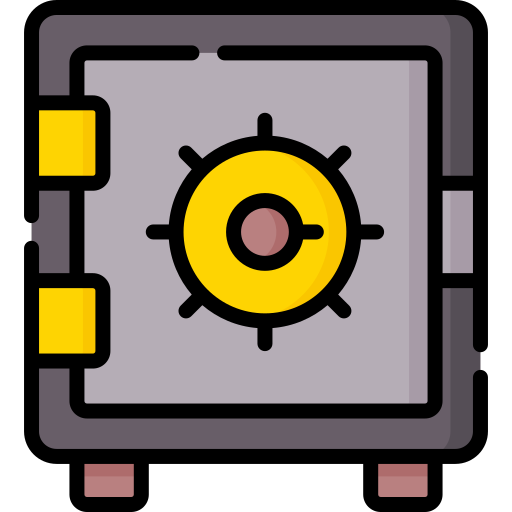
\includegraphics[width=0.25\textwidth]{docs/figs/safe.png}
    \caption*{Image courtesy of Flaticon.com \cite{flaticonSafeDeposit}.}
    \label{fig:safeIcon}
\end{figure}

\vspace{7cm}

\Large
\textbf{CS460: Software Engineering} \\

\end{center}
\end{titlepage}

\newpage

\tableofcontents

\newpage

\section{Introduction}
In today's homes, safes have become commonplace, and digital safes are increasingly favored by Americans for their convenience and heightened security features. Our product, HomeSafe, has been meticulously designed with the vigilant consumer in mind, catering to those who value convenience, security, and reliability. It distinguishes itself through a streamlined setup process, robust biometric two-factor authentication (2FA), user monitoring for access control, and an auxiliary power source. While mirroring the user experience of a typical digital safe, HomeSafe aims to encompass a unique set of features typically associated with commercial-grade safes. \\ \\
The Software Requirements Specification (SRS) provides a comprehensive insight into the features, external and internal interfaces, control logic, and design constraints of HomeSafe. The system employs a dynamic model based on the Object Modeling Technique (OMT) to direct and structure user interactions with the product, effectively governing the control flow within the system. \\ \\
As previously detailed in the Requirements Definitions Document (RDD), the core requirements formulated by the marketing team encompass multi-user capability, enhanced security via 2FA, user-friendly setup and maintenance, and continuous security and access. These fundamental requirements lay the groundwork for HomeSafe's development, guiding the organization of its components to achieve these objectives. The RDD outlines the capabilities and design constraints essential for realizing HomeSafe's overarching goals.

\section{Definition of Terms}
This section provides definitions for critical terms recurrently utilized throughout the document. This section can be a reference point for readers engaging with the content.

\begin{enumerate}
    \item[I.] \textbf{Administrator}: An individual with authority to establish and oversee separate user profiles within the system, regulating user access to the system's settings and contents.
    \item[II.] \textbf{Auxiliary}: An additional or secondary power source that supports the main or primary power supply. An auxiliary power source is typically used to provide backup, redundancy, or temporary power when the main power source is unavailable, disrupted, or insufficient.
    \item[III.] \textbf{Bio-Metric Scanner}: A technology that identifies and authenticates users based on their unique biological characteristics, typically fingerprints, retina patterns, or other traits.
    \item[IV.] \textbf{Microcontroller}: A microcontroller is a small integrated circuit serving as the central processing unit (CPU) of a safe's electronic system. It contains a processor, memory, and input/output ports and can include programmable capabilities. Microcontrollers manage the safe's tasks, user input, security protocols, and control functions, including locks, interface interactions, and external device communication.
    \item[V.] \textbf{Personal Identification Number (PIN)}: A numerical code that serves as a security credential used to authenticate and verify the identity of an individual. PINs are commonly used in various systems, such as electronic devices, bank accounts, and access control systems, to ensure that only authorized users can gain access.
    \item[VI.] \textbf{Two-Factor Authentication (2FA)}: A security protocol that requires users to provide two distinct forms of verification to access a system. This commonly involves a combination of something known (such as a password) and something possessed (such as a generated code or biometric information), adding an extra layer of security and protection against unauthorized access \cite{identityautomationTwoFactorAuthentication}.
\end{enumerate}

\section{General Description}
At the core of our software architecture lies the microcontroller, serving as the pivotal component responsible for overseeing all of HomeSafe's operations. This microcontroller is the nexus, intricately linked to all the physical elements housed within HomeSafe. It adeptly manages inputs from various input devices and orchestrates the delivery of corresponding outputs to designated output devices. To enable its functionality, the microcontroller is programmed using our custom-developed software, ensuring the precise execution of desired operations.

\newpage

\begin{figure}[h]
    \centering
    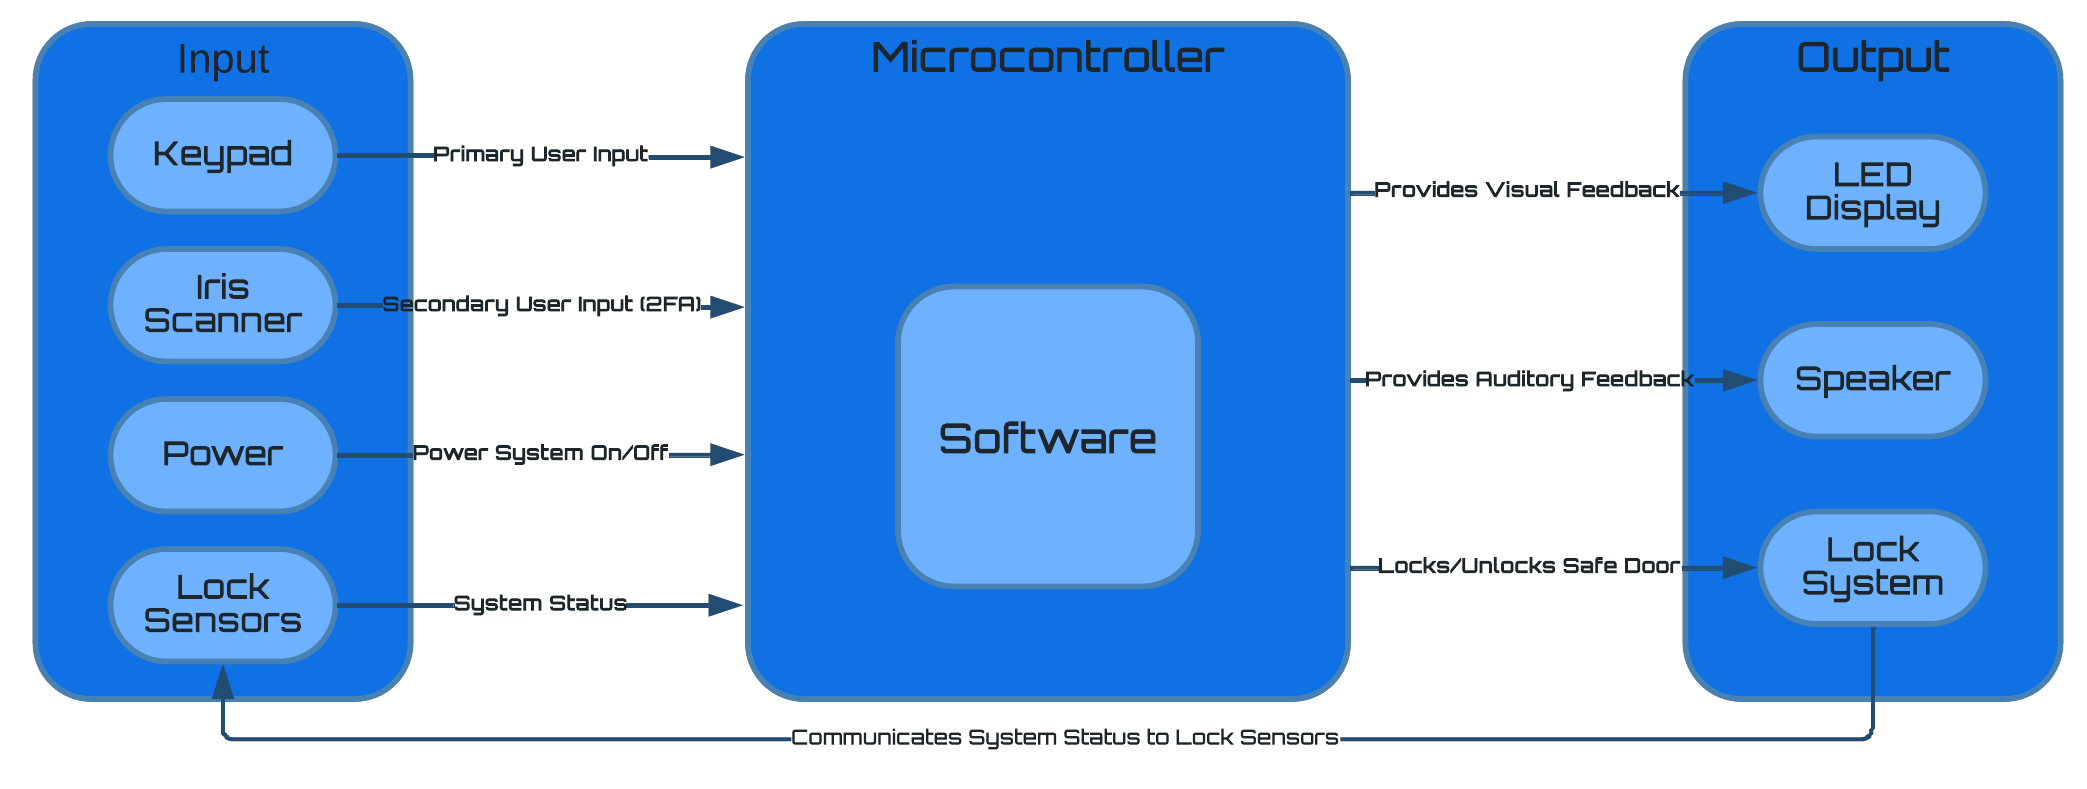
\includegraphics[scale=0.32]{docs/figs/system_diagram.png}
    \caption{Block Diagram of HomeSafe System \cite{lucidLucidVisual}}
    \label{fig:diagram1}
\end{figure}

\begin{itemize}
    \item \textbf{Keypad}: The software permits users to enter their assigned PIN using the numeric keys 0-9. Any key press triggers the LED display screen and speaker to offer visual and auditory feedback. Upon successful identity verification via the correct passkey, the software sends a signal to the microcontroller, activating the iris scanner for two-factor authentication (2FA). After inputting the entire PIN, the user must press the ENTER button to initiate password verification. In the case of an erroneous number entry during PIN input, the user can press the CANCEL button to abort the entry attempt and reset the procedure.
    \item \textbf{Iris Scanner}: The software allows users to input data through the Iris Scanner after successfully verifying the PIN. After completing the PIN verification, the system will prompt the user for an iris scan. Once the iris scan is completed and the user's identity is confirmed, access to the safe is granted. Visual and auditory notifications are provided through the LED Display and Speaker, and a signal is sent to the Lock System to switch the safe's status from LOCKED to UNLOCKED.
    \item \textbf{Power}: When you press this button, the system will initiate, showing the main menu for PIN input on the LED Display. A startup sound will also emanate from the Speaker, signaling the user that the system is operational. It's important to note that the system can only be powered off when in the LOCKED state. If the user tries to power off the procedure while in this state, a warning message will be displayed on the LED screen.
    \item \textbf{Lock Sensors}: The interface tasked with conveying the current status of the HomeSafe (whether in the LOCKED or UNLOCKED state) to the microcontroller.
    \item \textbf{LED Display}: The LED (Light Emitting Diode) display is a visual interface for user interaction. Its primary role is to initiate user input and, when input is made via the keypad, to provide feedback by indicating the current number of characters entered. Furthermore, it can convey additional information, such as system warnings or low-power notifications, to the user.
    \item \textbf{Speaker}: A micro-speaker is integrated into the HomeSafe to convey auditory feedback to the user when buttons are pressed.
    \item \textbf{Lock Mechanism}: This system's role is to authorize entry into the HomeSafe once user authentication is completed. Upon successful authentication, the microcontroller transmits a signal to the lock mechanism, releasing the latch and making the door accessible for the user to open. This system also communicates with the Lock Sensors, which transmit this information to the software and allow further operation.
    
\end{itemize}

\section{Specific Requirements}
In this section, we take a deep dive into the inner workings of the system logic and how it reacts to the full spectrum of user interactions. We'll uncover how our software interprets and handles these interactions, giving you a clear picture of how HomeSafe smoothly manages its operations in response to diverse user actions and inputs.

\begin{figure}[!h]
    \centering
    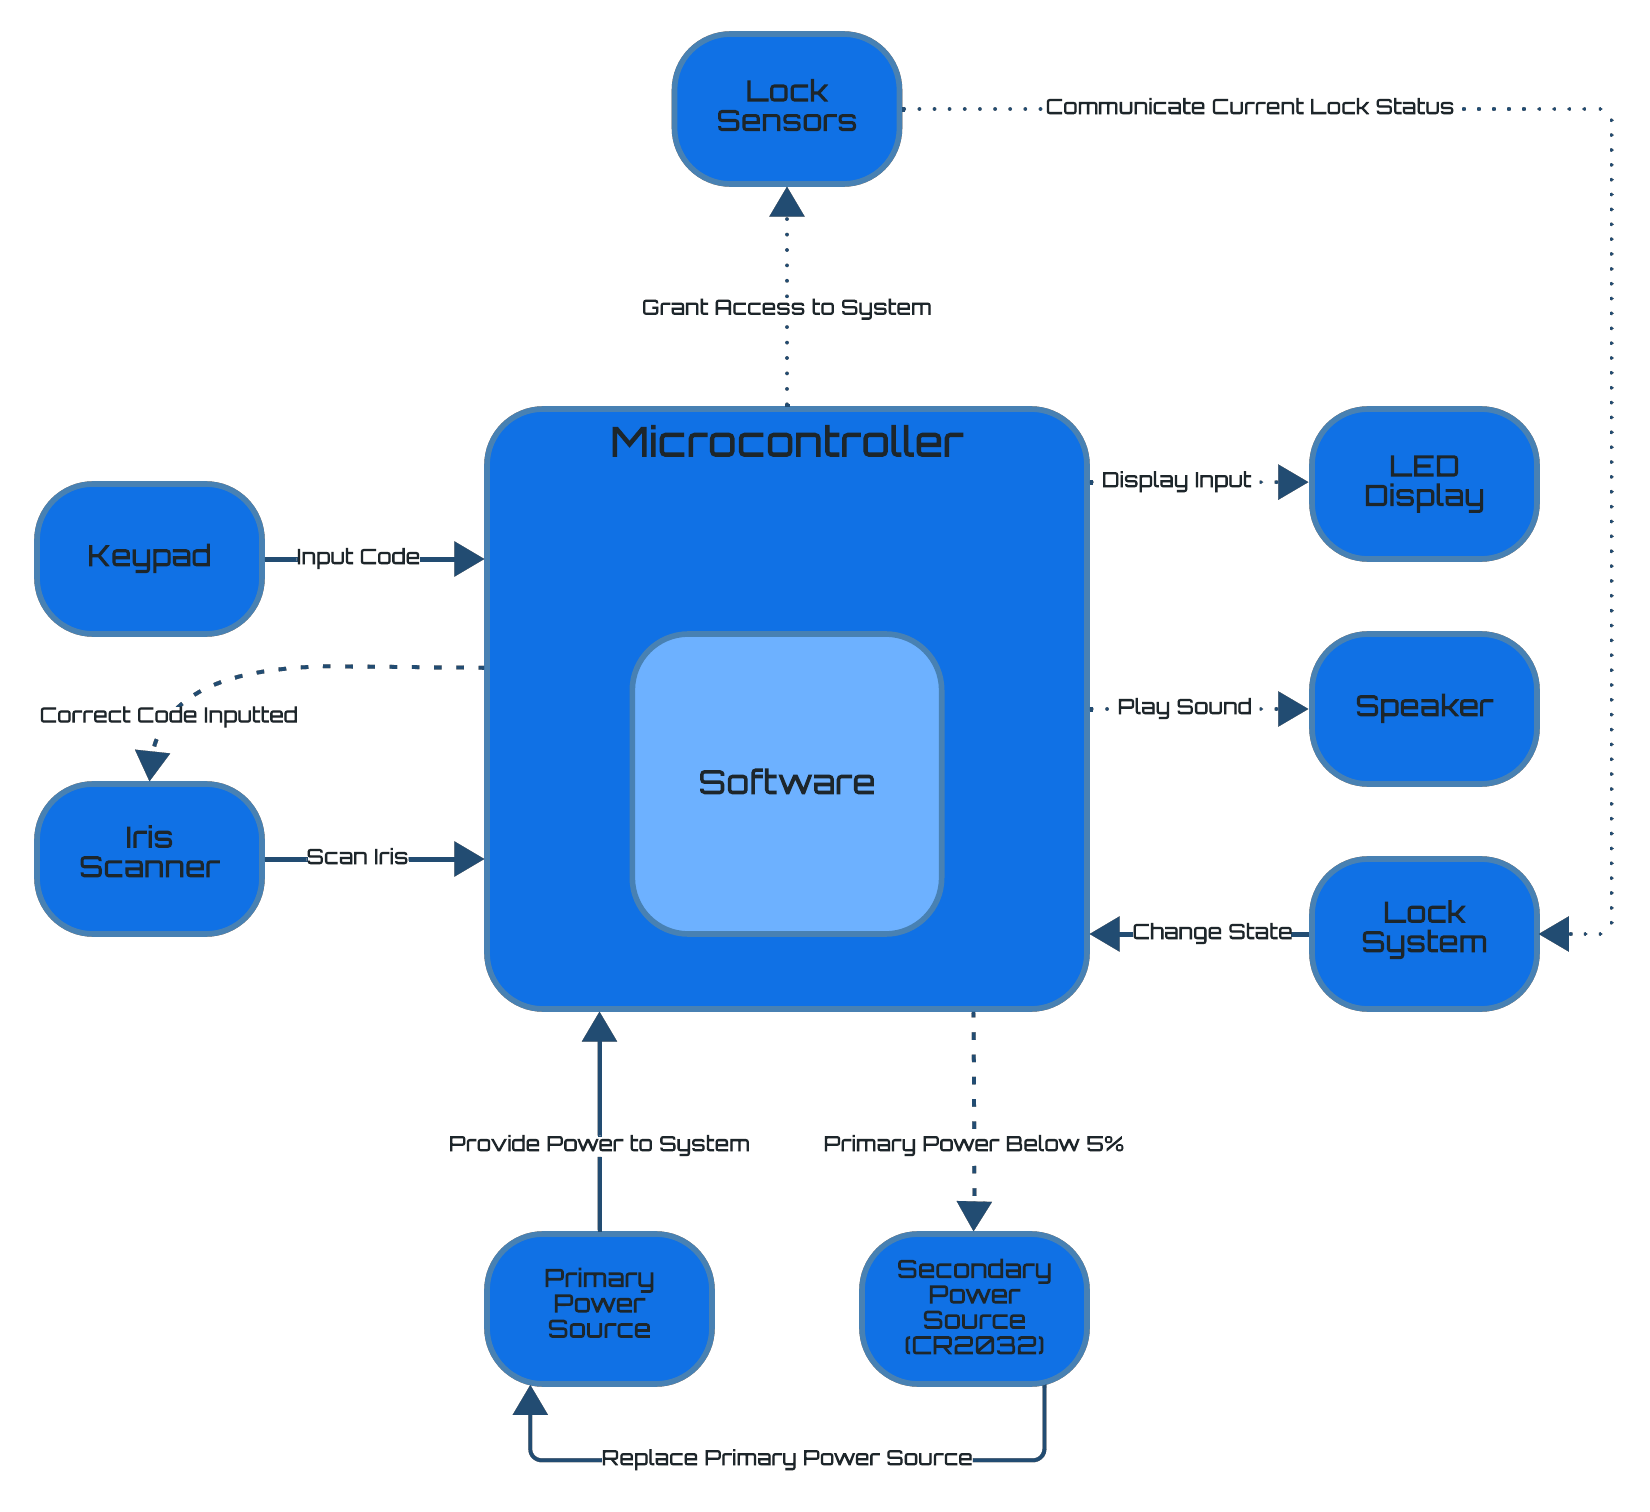
\includegraphics[scale=0.3]{docs/figs/logical_diagram.png}
    \caption{Logical Diagram of HomeSafe System \cite{lucidLucidVisual}}
    \label{fig:diagram2}
\end{figure}

\subsection{External Interfaces}
The software residing on the microcontroller governs all communication between the input and output components. Figure 2 provides a graphical representation of the physical input channels and the feasible output channels they can activate. Section 3.1 elaborates on the dynamics of interactions occurring between these inputs and outputs, while Section 3.2 illustrates the system's control flow using transition-state models.

\subsubsection{Input Events}
The interaction between users and the safe is facilitated through the keypad, iris scanner, and lock sensors, each serving a vital role in ensuring security and accessibility.

\begin{itemize}
    \item \textbf{Keypad}: Users can input their designated PIN using the software's number keys from 0-9 for identity verification. Every keypress triggers both visual and sound responses from the LED screen and speaker. When the correct PIN is entered, the software communicates with the microcontroller, initiating the iris scanner for an added layer of two-factor authentication (2FA). After entering their entire PIN, users must press the ENTER button to validate. \textbf{Note}: For added security, an '*' appears on the screen with each number keypress to ensure privacy, especially if someone is nearby.
    \item \textbf{Iris Scanner}: This system represents the second user authentication layer. After successful PIN verification, the software allows users to input data through the Iris Scanner. After validating the PIN, the system prompts the user for an iris scan. Upon the successful completion of the iris scan and the subsequent confirmation of the user's identity, access to the safe is authorized. Visual and auditory notifications are provided through the LED Display and Speaker to enhance user understanding and engagement. Simultaneously, a signal is dispatched to the Lock System, orchestrating the transition of the safe's status from LOCKED to UNLOCKED, ensuring a robust and multi-tiered security approach.
\end{itemize}

\subsubsection{Output Events}
The channels where the safe interacts with the input mechanisms are the LED Display, Speaker, and Lock System.
\begin{itemize}
    \item \textbf{LED Display}: The LED display serves as a visual interface for user interaction, primarily initiating input and providing character count feedback when using the keypad. Additionally, it communicates important system information, such as warnings and low-power notifications, to the user.
    \item \textbf{Speaker}: A micro-speaker is seamlessly integrated into the HomeSafe, designed to deliver auditory output events to the user in response to button presses.
\end{itemize}

\subsection{Internal Interfaces}
This subsection delves into the essential internal components that make the system function seamlessly: the microcontroller, software, locking mechanism, and lock sensors.

\subsubsection{Microcontroller}
Serving as the system's central intelligence hub, the microcontroller is powered by the batteries and acts as the core decision-making unit. It receives and interprets various inputs, ensuring they are processed accurately before conveying any corresponding output to the user. In addition, the microcontroller requires power to store and manage crucial user data, including PINs and biometric information, contributing to the system's robust security framework.

\subsubsection{Software}
The software is the critical bridge between the user and the system's hardware components. It operates with the microcontroller to manage user interactions and authentication processes. The software ensures that the user's input is processed correctly, and it facilitates communication between the various hardware components to provide a seamless and secure user experience.

\subsubsection{Lock Mechanism}
The lock mechanism's primary role is granting entry into the HomeSafe once user authentication is completed. Upon successful authentication, the microcontroller, in conjunction with the software, transmits a signal to the lock mechanism, effectively releasing the latch and permitting the user to access the contents of the safe.

\subsubsection{Lock Sensors}
Integral to the security of the HomeSafe, the lock sensors continuously monitor the status of the safe's door, accurately detecting whether the locking mechanism is in a locked or unlocked state. This crucial information is communicated to the microcontroller and software, ensuring real-time awareness of the safe's security status and allowing the system to respond promptly to user actions and the safe's condition.

\subsection{Control Logic}
The control flow of the system orchestrates various operations to ensure the secure and efficient functionality of the safe. This section outlines the process of setting up initial user credentials and subsequent actions within the system.

\subsubsection{Initial Setup Process}
This section delineates how users set their PIN and input their iris scan to secure access to the safe. Upon receipt, the safe remains locked but is energized by a functioning battery and features an active keypad. The individual endowed with the master PIN, supplied with the safe, assumes the administrator role. \\ \\
Enclosed with the safe is a user guide, the final page prominently displaying a unique 6-digit master PIN. On powering up the safe for the first instance, users are guided to input this master PIN to kickstart their credential configuration. After the master PIN's successful recognition, users are ushered to determine their 6-digit PIN. After setting this PIN, the system beckons for an iris scan to bolster the authentication process. After successfully capturing the iris scan, the user profile is constituted, and the data is anchored securely to the microcontroller. \\ \\
Having successfully registered the personal PIN and the iris scan, the safe affords access, preserving the user's details with utmost confidentiality. Crucially, the master PIN facilitates the preliminary setup and is a lifeline for recovery should a user misplace their PIN. Upon wrapping up the initial setup, this configuration mode is sealed within the microcontroller, and reverting or altering it demands intervention from the manufacturer.

\begin{figure}[!h]
    \centering
    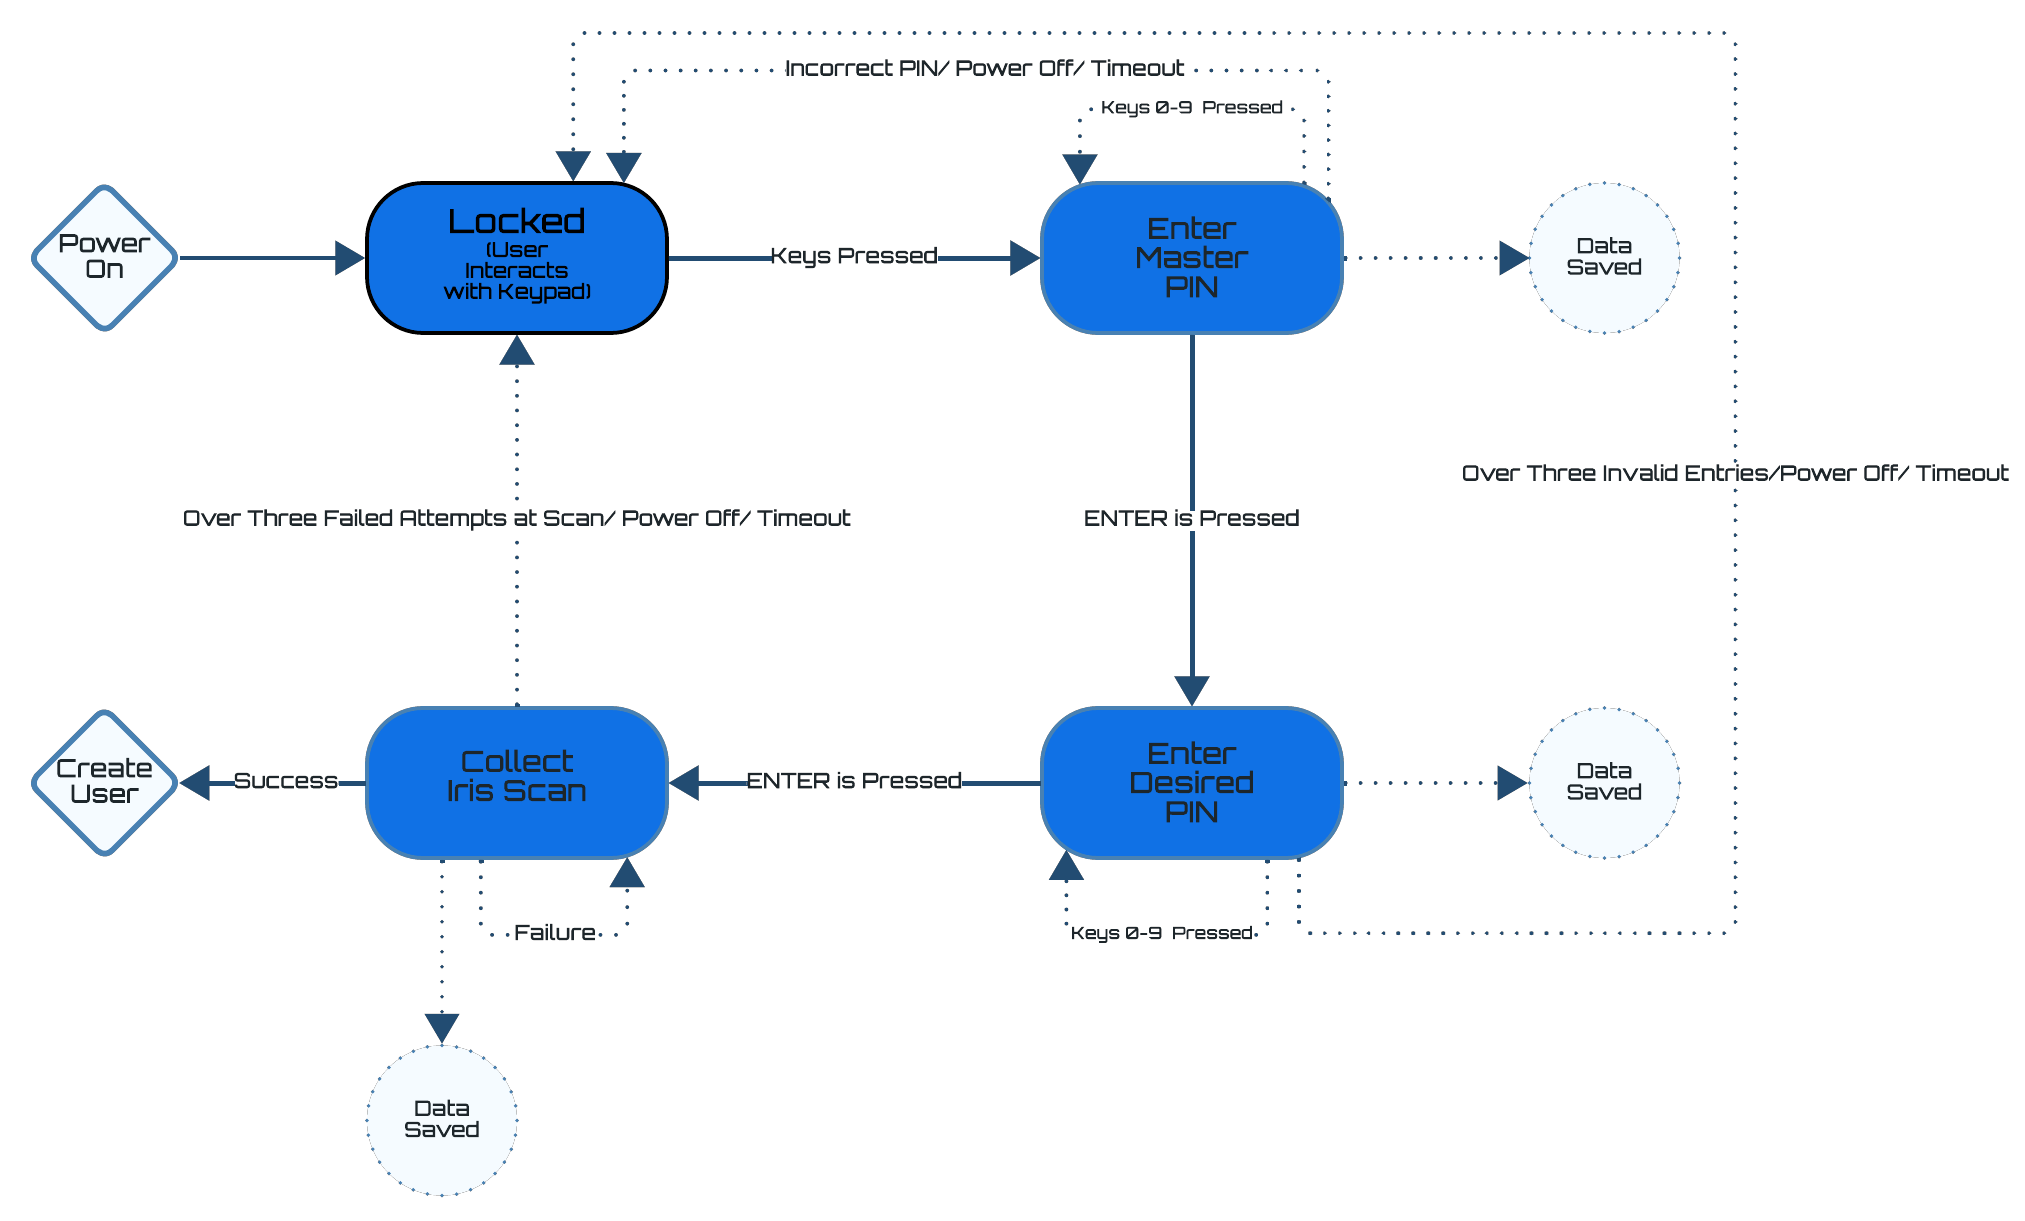
\includegraphics[scale=0.28]{docs/figs/initial_setup.png}
    \caption{Dynamic OMT Diagram of the Initial Setup Process \cite{lucidLucidVisual}}
    \label{fig:diagram3}
\end{figure}

\subsubsection{Authorization}
In the framework of control logic, this section steers through the pivotal steps required for users to gain authorization to the safe. The process initiates with a secured door fronted by an active keypad. To kick off the authentication, users power on the safe and key in their 6-digit PIN. Following the system's acknowledgment of the entered PIN, the subsequent stage ushers in the Iris Scanner - a lynchpin in ensuring advanced authentication. \\ \\
Users are then prompted to provide a single iris scan through the scanner interface. The system securely stores and cross-references this captured scan during subsequent access attempts. In scenarios where a user's iris scan doesn't match the saved data, or if unsuccessful matching ensues thrice in a row, the safe enforces a one-hour lockout. Persistent lockouts necessitate the intervention of the master PIN to reaccess the safe, ensuring an elevated layer of security, thereby making it virtually impregnable.

\begin{figure}[h]
    \centering
    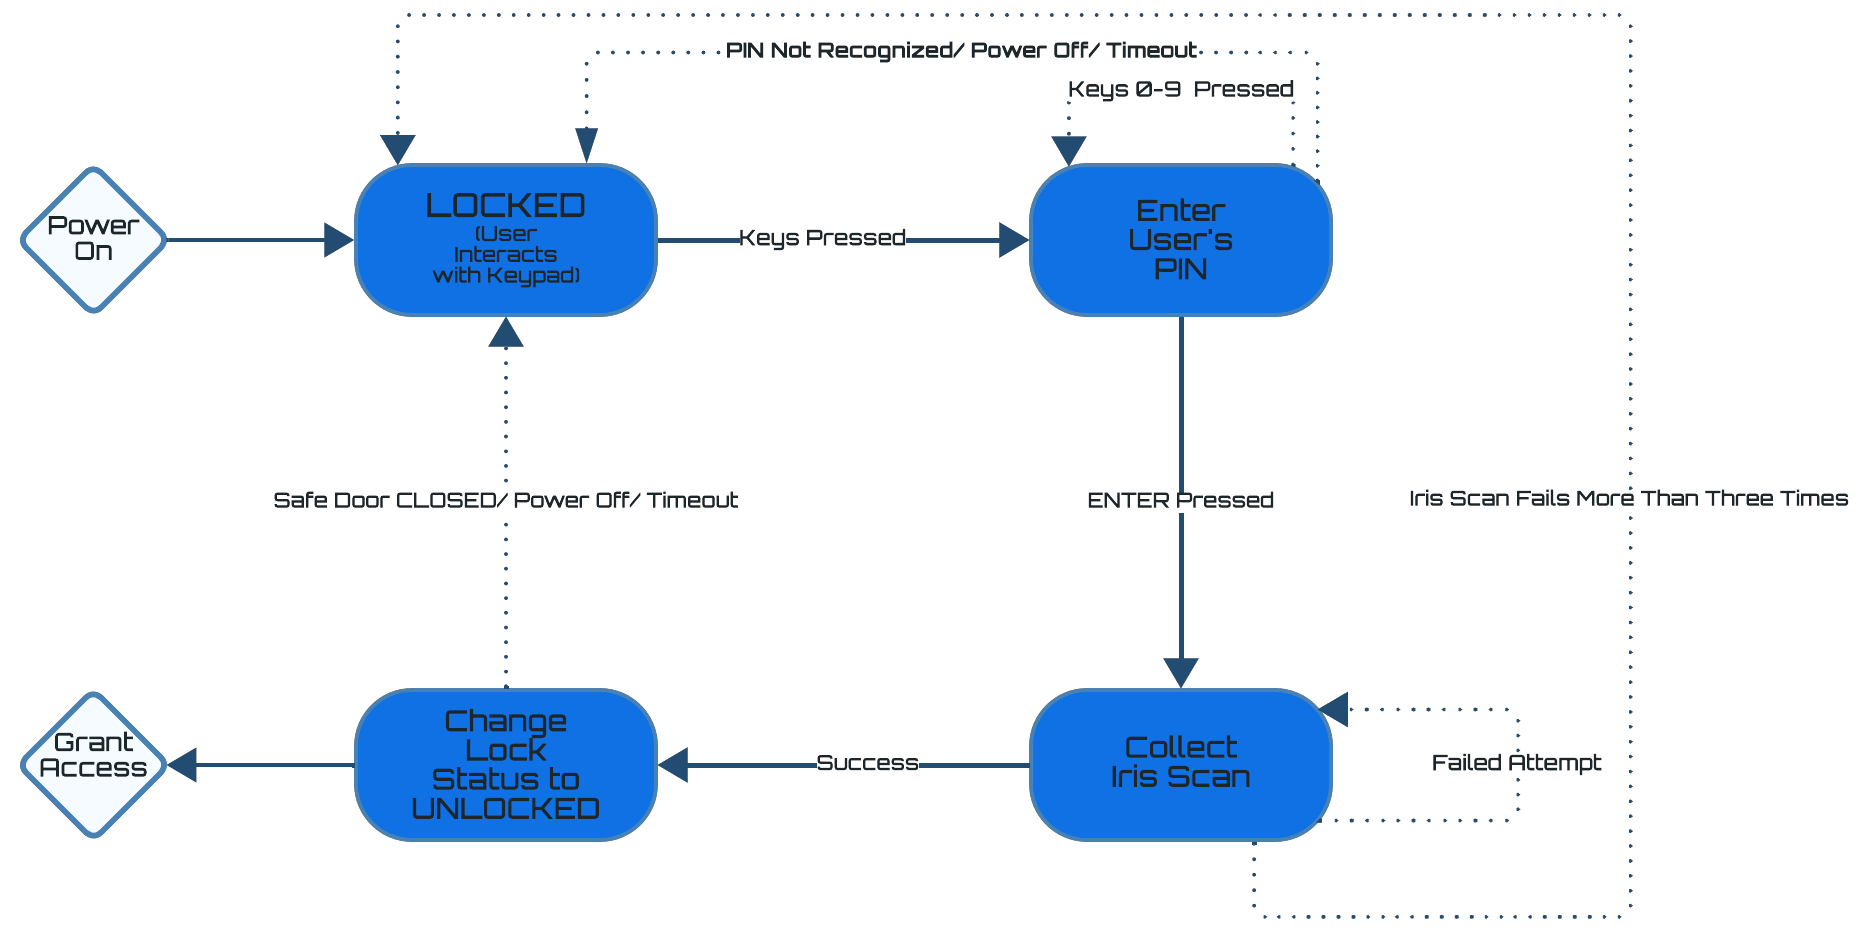
\includegraphics[scale=0.28]{docs/figs/authorization_process.png}
    \caption{Dynamic OMT Diagram of the Authorization Process \cite{lucidLucidVisual}}
    \label{fig:diagram4}
\end{figure}

\newpage

\section{Design Constraints}

\begin{itemize}
    \item The control software for HomeSafe is crafted using Java, which means it operates within the confines and opportunities presented by an object-oriented programming language. This choice of language enables a structured and modular design approach, allowing for the efficient management of complex system behaviors. However, it also implies certain limitations associated with Java-based applications' performance and resource utilization.
    \item The auxiliary power supply, a single CR2032 cell battery, can sustain the system for an estimated ten years \cite{microbatteryEverythingNeed}. However, suppose the additional power supply depletes before the primary power source is reinstated (two non-rechargeable alkaline AA batteries). All user data will be forfeited, rendering the unit's contents inaccessible. Additionally, due to the microcontroller's exclusive control over the lock mechanism, manual operation of the safe box is not feasible. Consequently, should both the primary and secondary power sources fail, none of the users will possess the means to access HomeSafe.
    \item The HomeSafe is 12 x 16 x 12 inches (L x W x H). This may limit how much the customer can store inside.
\end{itemize}

\newpage

\printbibliography

{\parindent0pt}

\end{document}
